\section{Introduction}
In this project we have analized the behaviour of the implementation of an FPU \cite{mor1kxcode} provided by our professor with the aim of optimize the number of cycles and the operating frequency.


\subsection{Problem statement}
The goal of the project was to optimize the FPU shipped with the mor1kx from the point of view of the number of clock cycles required by each operation. In particular, we were required to reduce the number of clock cycles needed to compute addition, subtraction, multiplication and conversion from integer format (with two's complement) to floating point IEEE 754 (32 bit), and viceversa.

In order to do this, we were given a working implementation and, starting from it, we tried to move pieces of computation in different stages, with the constraint of a minimum clock frequency of 140MHz (clock period of 7 ns).

The original implementation of the FPU was composed of 7 modules: add/sub, mul/div, i2f conversion, f2i conversion, compare, rounding and the top module. In the top module there were some computations, which were useful to prepare the computation of all the other modules. In particular, the top module checks which operation should be performed, splits the input signals in sign, exponent and mantissa, and computes some special cases (infinite, invalid, zero input).
In particular, all the outputs of the modules related to the operations were given in input to the rounding module, which was the final module generating the three output signals of the FPU (fpu\textunderscore arith\textunderscore valid, fpu\textunderscore result, and fpcsr\textunderscore o). The initial operating frequency of the FPU was 100MHz, i.e. a clock period was 10ns.

\textbf{\prettyref{tab:firstTiming}.}


\begin{table}
\small
\begin{center}
\caption{Summary of clock cycles required for each operation in the original implementation}

\begin{tabular}{@{}|c|c|@{}}
\toprule
\textbf{Operation    }                                                & \multicolumn{1}{l|}{\textbf{Clock cycles}} \\ \midrule
Compare                                                      & 1                                 \\ \midrule
Add/sub                                                      & 6                                 \\ \midrule
Multiplication                                               & 7                                 \\ \midrule
Division                                                     & 19                                \\ \midrule
ITOF                                                         & 4                                 \\ \midrule
FTOI                                                         & 4                                 \\ \midrule
Rounding(already included in the count above except compare) & 2                                 \\ \bottomrule
\end{tabular}
  \label{tab:firstTiming}
\end{center}
\end{table}

\subsection{Background}
\textbf{IEEE 754 Single Precision}
\newline

This is a standard representing floating point numbers on 32 bits. These bits are divided in Sign (S, 1 bit), Exponent (E, 8 bits) and Mantissa, which is the fractional part (M, 23 bits). The number is usually represented in a normalized form, i.e. it is written as $1.(M) * {2}^E $ , thus only the fractional part is represented in M. Regarding, the exponent E, it could be also negative: in order to represent only positive exponents, the standard adds a bias of 127 before representing the exponent in the final result. Amoung the 256 different possible exponents, the value 0 is reserved for zero and denormalized results, while the value 255 is reserved for NaN and infinite values. This means that, if 1 <= E <= 254, the represented number is $ F=(-1)^S * (1.M) * {2}^{(E-127)}$ .
\newline

\textbf{CONVERSION FROM INTEGER TO FLOAT}
\newline

The conversion form Integer to Float takes an integer number represented in two's complement, and computes the sign. In case of a negative number, takes the module and computes the exponent. After the exponent computation, shifts right the input number (reducing the size from 32 to 24 bits). At this pont, we can compose the result putting together the sing, the biased exponent, which is the exponent plus 127, and the fractional part, without considering the hidden bit.
\newline

\textbf{CONVERSION FROM FLOAT TO INTEGER}
\newline

In the floating to integer conversion we start with a 32 bits number, then this number is split into sign, exponent (8 bits) and mantissa (23 bits). We then convert the exponent into decimal and subtract the bias (in ieee 754 single precision this bias is 127).
We add the implicit 24th bit to the mantissa, in this way each bit represents a value, starting at 1 and halves for each bit, as follows: bit 23 = 1, bit 22 = 0.5, bit 21 = 0.5 and so on. We can now decode the significand by adding the values represented by these bits. Once we have computed this values we need to multiply with the base 2, to the power of the exponent, to get the final result.
\newline

\textbf{ADDITION/SUBTRACTION}
\newline

The floating point addition/subtraction is implemented using the basic algorithm: first, we compute the difference between the exponents in order to detect the greates operand d=Ea-Eb. Then shift the smallest one 'd' positions to the right (aligning it to have the same exponent). At this point, perform the needed operation on the fractional parts:
\begin{itemize}
\item in case of a ADD, sum the fractionals if they have the same sign, else subtract them;
\item in case of a SUB, sum the fractionals if they have different sign, else add them.
\end{itemize}
Atfer computing the sum, perform normalization:
\begin{itemize}
\item if the result is already normalized, no further operation needed;
\item in case we are adding the fractionals, we can have 2 leading bits before the ".", in this case, right shift of 1 position the fractional, and increase the exponent by one;
\item in case we are subtracting the fractionals, we can have 'n' leading zeros, hence shift left of n positions the fractional and decrease the exponent by n.
\end{itemize}
After normalization, we can round according to the specified rounding mode and generate the flags on the result, signaling possible exceptions.
\newline

\textbf{MULTIPLICATION}
\newline

The algorithm used for the multiplication is the following one. Regarding the mantissas of the two operands, they are multiplied considering also the hidden bit. For the exponent, we sum the unbiased exponents, and then we add again the bias (+ 127) for correct representation in the standard. At this point, we put the results together (sign, biased exponent and mantissa) adding the hidden bit.
After this, we need to dernomalize, shiftng the significand 1 place o the right, increasing the exponent by 1. The last operation is rounding depending on the desired rounding mode.
\newline


\subsection{Summary of the work}
We considered 4 operations: floating point addition/subtraction, multiplication (splitting multiplication from division, which was not required by the project), and conversion, from integer to floating point IEEE754 representation and viceversa. We optimized these operations, reducing the number of needed cycles (from the rising edge of the new\textunderscore fpu\textunderscore data to the rising edge of the fpu\textunderscore arith\textunderscore valid\textunderscore o), having as a constraint the maximum clock period of 7ns. In order to do this, we eliminated some stages, anticipating computation in the previous stages, or delaying it in the following ones.

In particular:
\begin{itemize}
 \item for the addition/subraction we optimized from 5 to 4 clock cycles;
 \item for multiplication, we moved from 7 to 4 c.c;
 \item for the conversions, we moved from 4 to 3 cycles.
\end{itemize} 
It was possible to reduce both the number of clock cycles and the clock period (from 10ns to 7ns)  thanks to the fact that the implementation at 10ns had very large slack in each stage.


\pagebreak

\section{Design and implementation}
In the following description we will use the following convention/notation, first we will provide a theoretic description of our implementation and then we will provide between () the name of the signals regarding the description. In the top module most of the computation are performed for both the operands and so we use \&\& to separate the signal of input a and the signal of input b.
The algorithm described can be found here \cite{mor1kxRep}.
\newline

\textbf{
\prettyref{fig:top_schema} shows a flowchart regarding the top module.}
\newline

\begin{figure}
\centering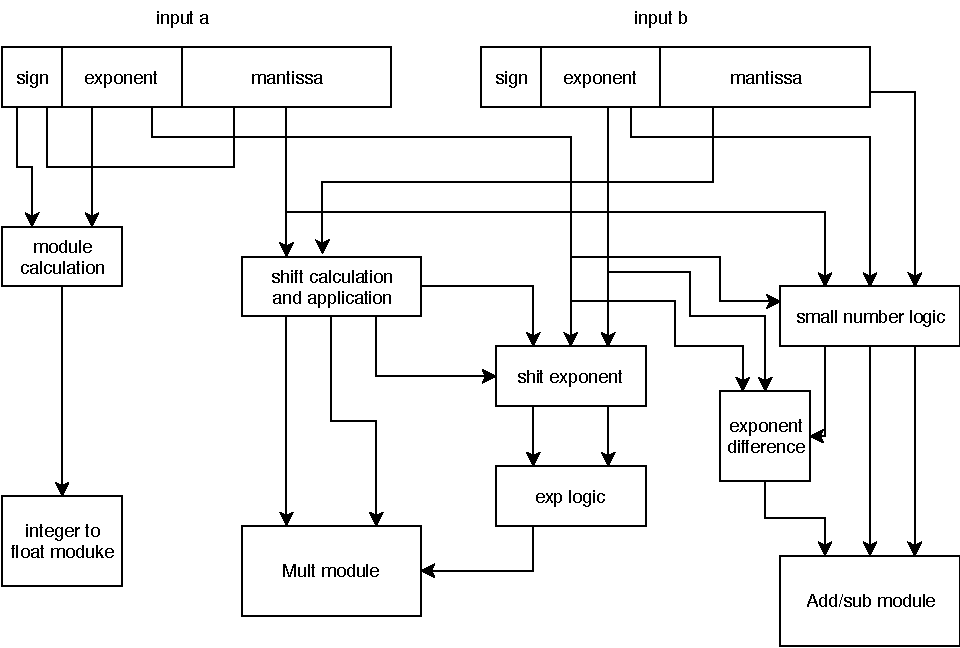
\includegraphics[width=15cm]{TopSchema}
\caption{Top flowchart}	
\label{fig:top_schema}
\end{figure}

\textbf{TOP}
\newline

The top module is the module containing all the other modules, in the original version this module was used just to execute some common calculations to all the operations such as the detection of infinite or nan cases. In our modified version we moved part of the computation of the single operations inside it in order to met timing constraints.
The top module receives as input the clock signal (clk), the reset (rst), the flush, which is used to cancel the current operation just like the reset (flush\textunderscore i), a signal that says if the operation can procede to the next stage of the computation in the top (padv\textunderscore decode\textunderscore i), a signal that says if the operation can procede to the next stage of the computation in the single module (padv\textunderscore execute\textunderscore i), a signal that is used to determine which type of operation the FPU must execute (op\textunderscore fpu\textunderscore i), a signal that describes the rounding mode that must be used (round\textunderscore mode\textunderscore i) and two 32 bits operand (opa\textunderscore i \&\& opb\textunderscore i).
As first operation we have a registering of top primary input, in this way we are able to avoid timing problems on the input, than we perform an analysis of input values: the 32 bits input are then splitted into sign, exponent and mantissa (for input a in\textunderscore signa, in\textunderscore expa, in\textunderscore fracta \&\& in\textunderscore signb, in\textunderscore expb, in\textunderscore fractb) and this values are used to determine if we have a special case like infinte, Nan, denormalized or zero input.
At this point we have some computation regarding the multiplication (and the future division), the integer to float conversion and the addition/subtraction. 
For the multiplication, after some precomputation on the exponent and on the mantissa in order to take in consideration the denormalized case, we calculate the number of leading zeros in the mantissa for both the operands (in\textunderscore nlza \&\& in\textunderscore nlzb ): these values are then used to shift the mantissa to obtain a mantissa with a 1 in the first position (in\textunderscore fract24a\textunderscore shl \&\& in\textunderscore fract24b\textunderscore shl). We also calculate the value of the exponent of the multiplication (in\textunderscore exp10mux). 

For the integer to float conversion we just calculate the module of the first input (in\textunderscore module\textunderscore a), since the second input is not used in this case, and we check if the input 'a' is zero (in\textunderscore opa\textunderscore 0).

For the addition and subtraction we determine which operand has the greatest exponent and the greater mantissa (exp\textunderscore gt, fract\textunderscore gt) and in a similar way we determine if the exponent and the mantissa are equal (exp\textunderscore eq, fract\textunderscore eq); this values are used to determine which is the greatest input value (addsub\textunderscore agtb) in order to establish which is the first operand (in\textunderscore fract24\textunderscore nsh) and which is the second one (in\textunderscore fract24\textunderscore fsh). We also use this values to determine the difference between the exponent (in\textunderscore exp\textunderscore diff).

The output are then set taking in consideration which is the operation performed by the FPU and in particular we set if the operation is valid (fpu\textunderscore arith\textunderscore valid\textunderscore o), the actual result (fpu\textunderscore result\textunderscore o) and some useful flags (fpcsr\textunderscore o).
\newline

\textbf{
\prettyref{fig:i2f_schema} shows a flowchart regarding the integer to float module.}
\newline

\begin{figure}
\centering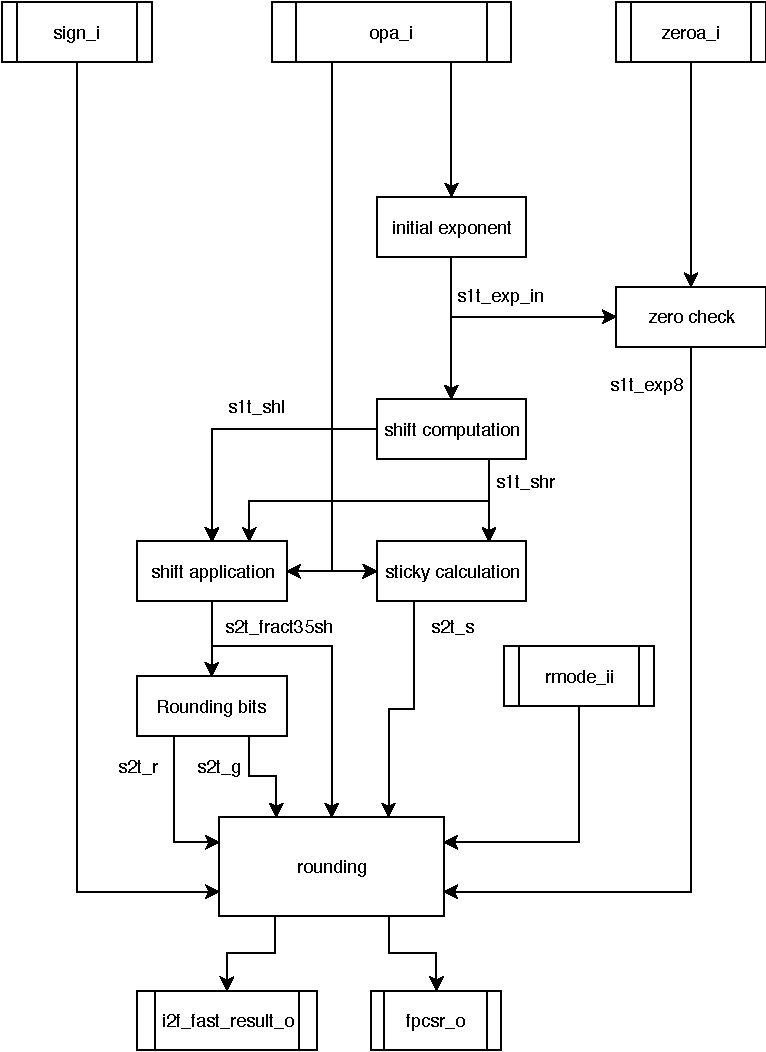
\includegraphics[width=15cm]{I2FSchema}
\caption{I2F flowchart}	
\label{fig:i2f_schema}
\end{figure}

\textbf{I2F}
\newline

The integer to float module receives as input the number to be converted into IEEE 754 floating point representation (32 bit opa\textunderscore i), the sign of the number (sign\textunderscore i) and a bit that signal if the input is zero (zero\textunderscore i), all the input are registered.
At this point we computed the position of the first one in order to calculate the correct exponent representation (s1t\textunderscore exp\textunderscore in). The value of the exponent is stored in a 8 bit variable: if the input number is zero, the exponent is set to zero, otherwise it is set as the sum of the position of the first one plus the bias of the IEEE standard (s1t\textunderscore exp8).
At this point we calculate the value of the possible right and left shift; if s1t\textunderscore exp\textunderscore in is greater than 23 it means that the most significant one is in one of the first 8 bit of the input (from the left) and the right shift could be at most 8 and the exact value is calculated as (s1t\textunderscore exp\textunderscore in - 23) and the left shift is zero; if s1t\textunderscore exp\textunderscore in is less than 23, the most significant bit is in one of the last 23 bit of the input (from the left) the left shift could be at most 23 in this case and the exact value is calculated as (23 - s1t\textunderscore exp\textunderscore in) and the right shift is zero (s1t\textunderscore shr and s1t\textunderscore shl).
We extend the input adding 3 bit in order to allow the calculation of the guard, round and sticky bit (s1t\textunderscore fract35).

At this point, using the value of the right shift we determine the sticky bit (s2r\textunderscore sticky); since the sticky bit in case of left shift equals to zero the final value of the sticky bit is exacly the sticky for the right (s1t\textunderscore sticky).
The sticky bit is calculated as the or bit-a-bit of those bits that are "lost" with right shift. 
The last operation of this first stage is the calculation of the shifted input accordly to the shifts previously calculated; the shifts are applied giving the priority to the right shift (s1t\textunderscore fract35sh).

The following values are than registered to the next stage: the sign of the input, the exponent, the input shifted, the sticky bit and the rounding mode.

We determine some flags depending on the rounding mode received (rm\textunderscore nearest, rm\textunderscore to\textunderscore zero, rm\textunderscore to\textunderscore infp, rm\textunderscore to\textunderscore infm) and we assign the value received from the previous stage.
Using the shifted input we calculate the guard, round, sticky and lost bit (s2t\textunderscore g, s2t\textunderscore r, s2t\textunderscore s, s2t\textunderscore lost) which are used to establish if the shited input must be rounded up (s2t\textunderscore rnd\textunderscore up). 

We round up in one of the following situation:
\begin{itemize}
 \item we round to the nearest and the sticky bit and the round bit are one or if the guard and the round and not the sticky;
 \item we round to the nearest and the sticky bit and the round bit are one or if the guard and the round and not the sticky;
 \item we round to the infinite negative and the lost bit is one and the sign of the input is negative.
\end{itemize}
The round is than applied to the first 32 bits of the shifted input ignoring the round bits (s2t\textunderscore fract32\textunderscore rnd).
The rounding phase could produce a variation of the exponent previously calculated, for this reason we update it taking in consideration the round (s2t\textunderscore f32\textunderscore exp10); the same reason apply to the mantissa (s2t\textunderscore f32\textunderscore fract24).
We than compose the result as: 1 bit for the sign, 8 bit for the exponent and 23 bit for the mantissa (s2t\textunderscore result) checking if the result is zero (s2t\textunderscore zero).
The result and the flags are then registered.
\newline

\textbf{
\prettyref{fig:f2i_schema} shows a flowchart regarding the float to integer module.}
\newline

\begin{figure}
\centering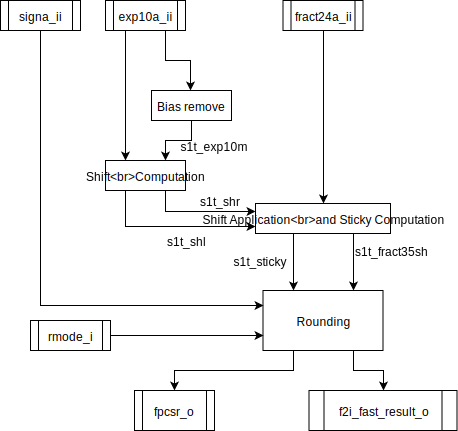
\includegraphics[width=15cm]{F2ISchema}
\caption{F2I flowchart}	
\label{fig:f2i_schema}
\end{figure}

\textbf{F2I}
\newline

The float to integer module receives as input the sign of the number (sign\textunderscore i), the exponent (exp10a\textunderscore i), the mantissa (fract24a\textunderscore i), a bit that signals if we have a sNan (snan\textunderscore i) and a bit that signals if the input is a qNan (qnan\textunderscore i), all the input are registered.

As first operation we subtract to the exponent received as input the costant 150, in this way we remove the bias and move the binary point at the end of the mantissa (s1t\textunderscore exp10m).
Than we calculate the possible right shift (s1t\textunderscore shr\textunderscore t) and we limit the possible shift up to 31 bits (s1t\textunderscore shr). In a similar way we determine if a left shift for the mantissa is required and we limit it to 15 bits (s1t\textunderscore shl). We check if the left shift is greater than (s1t\textunderscore is\textunderscore shl\textunderscore gt8) or equal to 8 (s1t\textunderscore is\textunderscore shl\textunderscore eq8); a left shift greater or equal than 8 will result in an overflow (s1t\textunderscore is\textunderscore shl\textunderscore ovf). 
The number received as input is than extended to 35 bits (f2i\textunderscore int35\textunderscore t) to take in consideration the shifts and, after a check on the right one to determine if it is zero (s1\textunderscore shr), we apply the shifts to it; the shifts are applied giving the priority to the right shift (s1t\textunderscore fract35sh). 
At this point, using the value of the right shift we determine the sticky bit (s2r\textunderscore sticky); the sticky bit is calculated as the or bit-a-bit of those bits that are "lost" with right shift.
In an equivalent way we calculated the possibile left shift (s1l\textunderscore sticky) and once both the two sticky bit are available we determine which one we will use in the rounding phase. Just like in the shifted input calculation we give the priority to the right one depending on the presence of the right shift (s1t\textunderscore sticky).

The following values are than registered to the next stage: the sign of the input verifing if we have a qnan or snan situation, the shifted number, two bit that rapresent the round and sticky bit,a bit that signals if the number is not valid, a bit rapresenting the sNan case, a bit rapresenting the overflow and the rounding mode.

We determine some flags depending on the rounding mode received (rm\textunderscore nearest, rm\textunderscore to\textunderscore zero, rm\textunderscore to\textunderscore infp, rm\textunderscore to\textunderscore infm) and using the shifted input, the round and sticky bit we calculate the lost bit (s2t\textunderscore lost), which is used with the guard, the round and the sticky bit to establish if the shited input must be rounded up (s2t\textunderscore rnd\textunderscore up).

We round up in one of the following situation:
\begin{itemize}
\item we round to the nearest and the sticky bit and the round bit are one or if the guard and the round and not the sticky;
\item we round to the infinite positive and the lost bit is one and the sign of the input is positive;
\item we round to the infinite negative and the lost bit is one and the sign of the input is negative.
\end{itemize}
The round is than applicated to the first 32 bit of the shifted input ignoring the round bits (s2t\textunderscore fract32\textunderscore rnd).

At this point we calculate some useful flags used to determine if an invalide case occured (s2t\textunderscore i32\textunderscore inv) and we calculate the two's complement in case of a negative number (s2t\textunderscore i32\textunderscore int32), futher that we check if the output number is zero (s2t\textunderscore i32\textunderscore int32\textunderscore 00).
The output is then assigned checking if we are in an invalid situation (s2t\textunderscore i32\textunderscore opc) .

The result and the flags are then registered.
\newline

\textbf{
\prettyref{fig:mult_schema} shows a flowchart regarding the multiplication module.}
\newline

\begin{figure}
\centering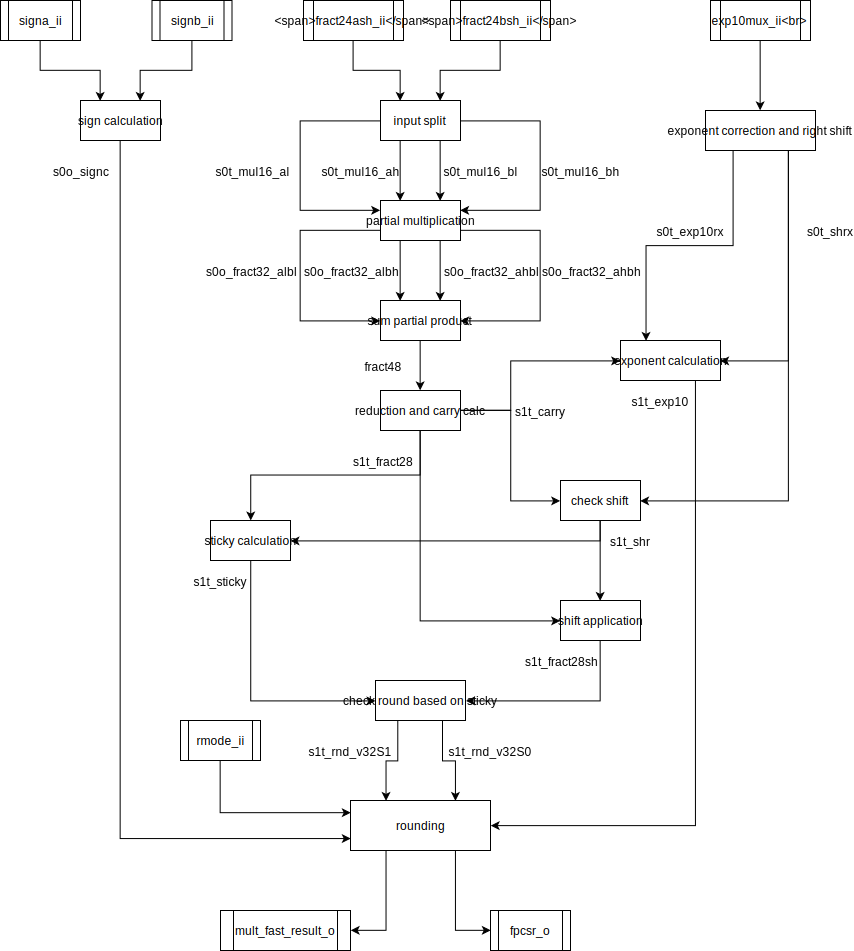
\includegraphics[width=17.5cm]{MultSchema}
\caption{Mult flowchart}	
\label{fig:mult_schema}
\end{figure}

\textbf{MULT}
\newline

The mul\textunderscore fast module receives as inputs the mantissa shifted left for both operands 'a' and 'b' (fract24ash\textunderscore ii and fract24bsh\textunderscore ii), such that the '1.' is in the most significant bit, the sign of the operands (signa\textunderscore ii and signb\textunderscore ii), some flags to detect invalid cases (snan\textunderscore ii, qnan\textunderscore ii, anan\textunderscore sign\textunderscore ii, inv\textunderscore ii, inf\textunderscore ii), a bit that says if at least one of the two operands is zero (opc0\textunderscore ii) and the exponent of the result (exp10mux\textunderscore ii). All these inputs are immediately registered.

In the first stage, we set to 0 the operands for actual multiplication (s0t\textunderscore fract24a and s0t\textunderscore fract24b) and the exponent of the result (s0t\textunderscore exp10c) if at least one of the operands is 0. Then we decompose the two operands in high and low part (s0t\textunderscore mul16\textunderscore al, s0t\textunderscore mul16\textunderscore ah, s0t\textunderscore mul16\textunderscore bl, s0t\textunderscore mul16\textunderscore bh), which will be used to compute the partial products. At this point, we compute possible right shift for the exponent and the corrected exponent (s0t\textunderscore shr\textunderscore t and s0t\textunderscore exp10rx), considering different cases. The right shift is limited by 31 (s0t\textunderscore shrx). 
At this point we register some flags related to exceptions on input values (s0o\textunderscore inv, s0o\textunderscore inf\textunderscore i, s0o\textunderscore snan\textunderscore i, s0o\textunderscore qnan\textunderscore i, s0o\textunderscore anan\textunderscore sign\textunderscore i) and some signals related to the multiplication computation: the sign of the result (s0o\textunderscore signc), the exponent of the result (s0o\textunderscore exp10c), the exponent for right shift (s0o\textunderscore exp10rx), the right shift (s0o\textunderscore shrx) and the partial products obtained by multiplying the two parts of each operand (s0o\textunderscore fract32\textunderscore albl, s0o\textunderscore fract32\textunderscore albh, s0o\textunderscore fract32\textunderscore ahbl, s0o\textunderscore fract32\textunderscore ahbh).

In the next stage, we have the computation of the resulting mantissa on 48 bits (fract48), obtained by summing up the four partial products obtained from the previous stage. Starting from the mantissa on 48 bits, we reduce it to 28 its, taking the 27 most significant bits and the or bit-a-bit of all the others (s1t\textunderscore fract28). Furthermore, we check if we have a carry (s1t\textunderscore carry). At this point we compute actual right shift and actual exponent of the result (s1t\textunderscore shr, s1t\textunderscore exp10).
Then, we apply a possible right shift, while we cannot have a left shift (s1t\textunderscore fract28sh), and we comput the sticky for no shift (s1l\textunderscore sticky). We determine some flags depending on the rounding mode received (rm\textunderscore nearest, rm\textunderscore to\textunderscore zero, rm\textunderscore to\textunderscore infp, rm\textunderscore to\textunderscore infm) and we assign the value received from the previous stage.

At this point we extend the fractional part to 32 bits (s1t\textunderscore fract32) for later calculations. We compute now the round (s1t\textunderscore r) and the guard bits (s1t\textunderscore g). Since the sticky computation is in the following stage, we compute some signals for both cases, i.e. sticky equal to 1 and equal to 0. Following this idea, we compute the lost bit in case of sticky equal to 0 (s1t\textunderscore lostS0), since in case of sticky equal to 1, the lost bit is the sticky iteself. Other signals that are computed in the two versions are the 'round up', detecting if we have to round up.

For the case of sticky equal to 1 (s1t\textunderscore rnd\textunderscore upS1), we round up in the following cases:
\begin{itemize}
\item we round to the nearest and the round bit is 1;
\item we round to the infinite positive and the sign of result is positive;
\item we round to the infinite negative and the sign of result in negative.
\end{itemize}

For the case of sticky equal to 0 (s1t\textunderscore rnd\textunderscore upS0), we round up in the following situations:
\begin{itemize}
\item we round to the nearest and both the guard and round bits are 1;
\item we round to the infinite positive, the sign of the result is positive and the lost bit in case of sticky equal to 0 is 1;
\item we round to the infinite negative, the sign of the result is negative and the lost bit in case of sticky equal to 0 is 1.
\end{itemize}

Following the computation of the rnd\textunderscore up bits in both cases, we decide if we have to add 1 to the fractional part, computing the values needed for rounding (s1t\textunderscore rnd\textunderscore v32S1, s1t\textunderscore rnd\textunderscore v32S0).
At this point, we perform a partial computation of the sticky bit, splitting the computation in two parts (s1t\textunderscore stickyh, s1t\textunderscore stickyl) and a signal telling us which part of the sticky we need (stickyfix): in case of a shift greater than or equal to 13, we will need both parts of the sticky, otherwise we will use only the first one.

Now we register some signals: flags related to exceptions on the input, the sign of the result, a signal telling us if a shift has been performed (s1o\textunderscore is\textunderscore shifted), the partial stickies, the exponent, the fractional part on 32 bit, the lost for sticky equal to 0 and the values needed for rounding

In the last stage, we compute the final sticky bit (s2r\textunderscore sticky) and the rounded fractional for both values of the sticky(s2t\textunderscore fract32\textunderscore rndS1, s2t\textunderscore fract32\textunderscore rndS0). At this point we can choose the actual fractional part on 32 bits of the result (s2t\textunderscore fract32\textunderscore rnd) depending on the sticky and the lost bit.
Then we compute the final exponent on 10 bits (s2t\textunderscore f32\textunderscore exp10) and the fractional on 24 bits (s2t\textunderscore f32\textunderscore fract24).
After this, we compute some useful flags and we compose the final result (s2t\textunderscore opc), giving priority to the exceptions. At the end of the module, these outputs are registered.
\newline

\textbf{
\prettyref{fig:add_schema} shows a flowchart regarding the addition/subtraction module.}
\newline

\begin{figure}
\centering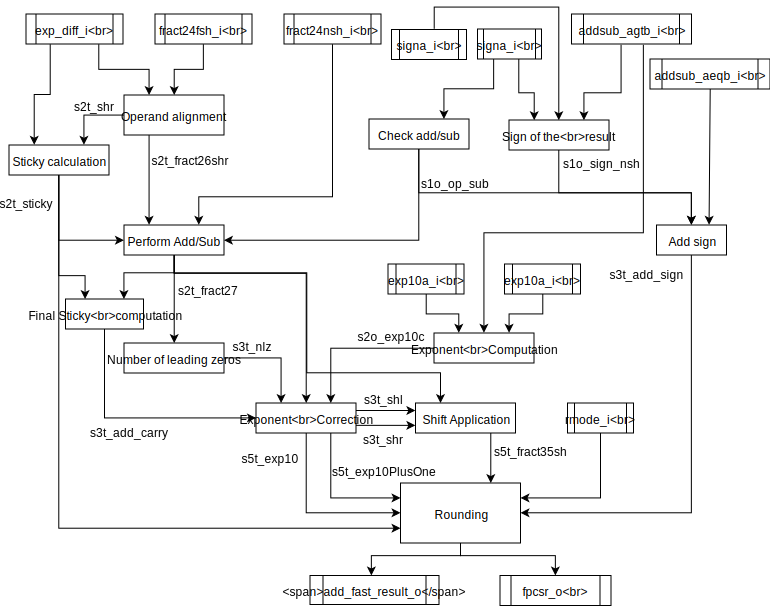
\includegraphics[width=15cm]{AddSchema}
\caption{Add flowchart}	
\label{fig:add_schema}
\end{figure}

\textbf{ADD/SUB}
\newline

This module receives as inputs the exponent of both the operands (exp10a\textunderscore i and exp10b\textunderscore i), some flags related to invalid inputs (snan\textunderscore i, qnan\textunderscore i, anan\textunderscore sign\textunderscore i,inv\textunderscore i, inf\textunderscore i), two signals which say if 'a' is greather than or equal to 'b' (addsub\textunderscore agtb\textunderscore i and addsub\textunderscore aeqb\textunderscore i), the mantissa of the two operands (fract24nsh\textunderscore i for the operand that doesn't need shift, and fract24fsh\textunderscore i for the operand that needs to be shifted), the difference of the exponents (exp\textunderscore diff\textunderscore i). All these input are registered, forcing the two mantissa to zero in case of an infinte input.

In the first stage, we comput the needed right shift (s2t\textunderscore shr), in order to have the same exponent for both the operands; then this shift is applied to the second operand after having extended it from 24 to 26 bits (s2t\textunderscore fract26\textunderscore shr). Using the extended operand (not shifted) and the right shift, we compute the sticky bit (s2t\textunderscore sticky): we use this bit to build a 28 bit mantissa for the second operand (s2t\textunderscore fract28\textunderscore shr) starting from the shifted one on 26 bits.
At this point, we can compute the addition (s2t\textunderscore fract28\textunderscore add): in case of a subtraction, we just add the first operand and the two's complement of the second one. We discard the least significant bit, taking only the first 27 bits (s2t\textunderscore fract27).
We register some signals: exeptions on the input, the sign of the result, the exponent, the mantissa on 27 bit, a flag saying if we have a subtraction and the result is 0 (s2o\textunderscore sub\textunderscore 0), the sticky (s2o\textunderscore sticky) and the round mode. Furthermore, we anticipate in this stage the final sticky for later computation in case of carry equal to 0 (s2o\textunderscore stickyFinalC0).

In the next stage, the first thing we compute is the left shift needed to normalize the result and the exponent for left shift (s3t\textunderscore shl and s3t\textunderscore exp10shl). The sign of the result is "fixed" in case we have a subtraction with 0 result and we are rounding to minus infinte (s3t\textunderscore add\textunderscore sign), and we extend the mantissa from 27 to 35 bits adding some zeroes and the sticky computed from the previous stage. We detect if there is a carry by taking the most significant bit of the mantissa on 27 bit (s3t\textunderscore add\textunderscore carry): at this point, we can have right shift at most equal to 1 in case of a carry equal to one (s3t\textunderscore shr), and we compute the corrected exponent for this case (s3t\textunderscore expPlusCarry). Now we can compute the final sticky (sticky), using the previous computed one (s2o\textunderscore stickyFinalC0) and the carry.
We register the sign of the result, the fractional part on 35 bits (s4o\textunderscore fract35), two conditions needed for next stage (s4o\textunderscore and\textunderscore condition\textunderscore 4 and s4o\textunderscore and\textunderscore condition\textunderscore 3), right and left shift, the carry, the two possible exponents, the final sticky and the rounding mode.

In the last stage, we determine some flags depending on the rounding mode received (rm\textunderscore nearest, rm\textunderscore to\textunderscore zero, rm\textunderscore to\textunderscore infp, rm\textunderscore to\textunderscore infm). We compute the final exponent (s5t\textunderscore exp10) ant the exponent plus one (s5t\textunderscore exp10PlusOne) for later use. Using this calculated exponents, we compute two signals telling us if they are greater than 254 testing the bits (condition\textunderscore notPlusOne and condition\textunderscore plusOne).
Now we apply the shift to the 35 bit fractional part, giving priority to the right shits due to the carry (s5t\textunderscore fract35sh). After this, we compute the guard, round, sticky and lost bits (s5t\textunderscore g, s5t\textunderscore r, s5t\textunderscore s and s5t\textunderscore lost) needed for rounding.

Given the flags for the rounding mode, we determine if we have to round up (s5t\textunderscore rnd\textunderscore up) in this cases:
\begin{itemize}
\item we round to the nearest and both round and sticky are 1;
\item we round to the nearest, guard and round bits are 1 while the sticky is 0;
\item we round to the infinite positive, the sign of the result is positive and lost is 1;we round to the infinite positive, the sign of the result is positive and lost is 1;
\item we round to the infinite negative, the sign of the result is negative and lost is 1.
\end{itemize}

At this point we compute the rounded fractional on 32 bit (s5t\textunderscore fract32\textunderscore rnd). We compute the final exponent (s5t\textunderscore f32\textunderscore exp10), choosing between the two previously computed values, and the condition telling us if the exponent is greater than 254, again choosing between the two previously computed (exponent\textunderscore condition). Then we take the final mantissa on 24 bit (s5t\textunderscore f32\textunderscore fract24) and check if we have a denormalized result (s5t\textunderscore f32\textunderscore fract24dn).

We calculate some flags regarding the result, we compose the final result (s5t\textunderscore opc) and at the end we register the result



\section{Experimental evaluation}
In order to check the functional correctness we tested, through a behavioural simulation using Xilinx Vivado, all the operations with 30 test cases for each rounding mode, comparing the results and corresponding flags (fpu\textunderscore result\textunderscore o and fpcsr\textunderscore o) given by our new implementation of the FPU, with the results given by the original implementation, verifing that the two results coincide. Results can be found here \cite{mor1kxtest}.
Through Vivado, we used Synthesizer to run synthesis and implementation, in order to analyize the timing of the various operations. The following results refer to the post-implmentation slack provided by Vivado. In particular, we analyzed the timing for the single operations and for our whole implementation of the Floating Point Unit.

\subsection{Experimental setup}
The software used to develop the project was Xilinx Viavado2018a.
The project has been implemented using an FPGA taken from the Artix-7 family, the xc7a100tcsg324-1, which is mounted on the Nexys4-DDR.

\subsection{Results}
Here we provide the result of our design, in particular we will provide both the number of clock cycles for each implemented operation \textbf{\prettyref{tab:clockCycles}.} and the slack obtained in post-implementation setting the top on the top module.


\begin{table}
\small
\begin{center}
\caption{Number of cycles of our implemented design}

\begin{tabular}{@{}|c|c|c|@{}}
\toprule
\textbf{Operation}& \textbf{Clock cycles} & \textbf{Slack } \\ \midrule
Top, all operation together &              & +0.036 \\ \midrule
Add/sub                     & 4            & +0.009 \\ \midrule
Multiplication              & 4            & +0.194 \\ \midrule
ITOF                        & 3            & +0.331 \\ \midrule
FTOI                        & 3            & +0.899 \\ \bottomrule
\end{tabular}
  \label{tab:clockCycles}
\end{center}
\end{table}

\section{Conclusions and Future Works}
We were able to optimize the four operations, reducing the number of clock cycles and the clock period. 
Future works will consist in a reimplementation of all the modules, the optimization of the floating point division and its integration in the FPU, together with the module for the compare operation.
